% !TEX TS-program = xelatex
% !TEX encoding = UTF-8 Unicode
% !Mode:: "TeX:UTF-8"

%This file contains the LaTeX code of my laboratory report for my ICS II course.
%Author: 张作柏/Zuobai Zhang <17300240035@fudan.edu.cn>

% This is a simple template for a LaTeX document using the "article" class.
% See "book", "report", "letter" for other types of document.

\documentclass[12pt]{article} % use larger type; default would be 10pt

\usepackage[utf8]{inputenc} % set input encoding (not needed with XeLaTeX)

%%% Examples of Article customizations
% These packages are optional, depending whether you want the features they provide.
% See the LaTeX Companion or other references for full information.

%%% PAGE DIMENSIONS
\usepackage[top=1.05in, bottom=0.95in, left=0.90in, right=1.10in]{geometry}
%\usepackage{geometry} % to change the page dimensions
\geometry{a4paper} % or letterpaper (US) or a5paper or....
% \geometry{margin=2in} % for example, change the margins to 2 inches all round
% \geometry{landscape} % set up the page for landscape
%   read geometry.pdf for detailed page layout information

\usepackage{graphicx} % support the \includegraphics command and options

% \usepackage[parfill]{parskip} % Activate to begin paragraphs with an empty line rather than an indent

%%% PACKAGES
\usepackage{booktabs} % for much better looking tables
\usepackage{array} % for better arrays (eg matrices) in maths
\usepackage{paralist} % very flexible & customisable lists (eg. enumerate/itemize, etc.)
\usepackage{verbatim} % adds environment for commenting out blocks of text & for better verbatim
\usepackage{subfig} % make it possible to include more than one captioned figure/table in a single float
% These packages are all incorporated in the memoir class to one degree or another...

%%% HEADERS & FOOTERS
\usepackage{fancyhdr} % This should be set AFTER setting up the page geometry
\pagestyle{fancy} % options: empty , plain , fancy
%\renewcommand{\headrulewidth}{0pt} % customise the layout...
\lhead{}\chead{}\rhead{}
\lfoot{}\cfoot{\thepage}\rfoot{}

%%% SECTION TITLE APPEARANCE
\usepackage{sectsty}
\allsectionsfont{\sffamily\mdseries\upshape} % (See the fntguide.pdf for font help)
% (This matches ConTeXt defaults)

%%% ToC (table of contents) APPEARANCE
\usepackage[nottoc,notlof,notlot]{tocbibind} % Put the bibliography in the ToC
\usepackage[titles,subfigure]{tocloft} % Alter the style of the Table of Contents
\renewcommand{\cftsecfont}{\rmfamily\mdseries\upshape}
\renewcommand{\cftsecpagefont}{\rmfamily\mdseries\upshape} % No bold!
\usepackage{titletoc}
\titlecontents{section}
              [1.5cm]
              {\bf \large}%
              {\contentslabel{1.8em}}%
              {}%
              {\titlerule*[0.5pc]{$\cdot$}\contentspage\hspace*{0.6cm}}%
		   [\vspace{0.5em}]
\titlecontents{subsection}
              [1.8cm]
              {\normalsize}%
              {\contentslabel{2.0em}}%
              {}%
              {\titlerule*[0.5pc]{$\cdot$}\contentspage\hspace*{0.6cm}}%
		   [\vspace{0.4em}]
\titlecontents{subsubsection}
              [2.1cm]
              {\small}%
              {\contentslabel{2.5em}}%
              {}%
              {\titlerule*[0.5pc]{$\cdot$}\contentspage\hspace*{0.6cm}}%
		   [\vspace{0.4em}]


\usepackage[UTF8]{ctex}
\usepackage{fancyhdr}
\usepackage{enumerate}
\usepackage{indentfirst}
\usepackage{extramarks}
\usepackage{titling}
\usepackage{xcolor}
\usepackage{fontspec}
\usepackage[CJKbookmarks=true,colorlinks,linkcolor=black]{hyperref}
\setmainfont{Times New Roman}

%%% END Article customizations

%%% The "real" document content comes below...

%\title{\textbf{Digital Logic and Computer Design Report}}
\title{\textbf{KDD Cup 2012 Track 1解题报告}}
\author{张作柏\\17300240035}
%\date{} % Activate to display a given date or no date (if empty),
         % otherwise the current date is printed 

\usepackage{amsmath}
\newcommand\calD{\mathcal{D}}
\newcommand\XX{\boldsymbol{\mathit{X}}}
\newcommand\qq{\boldsymbol{\mathit{q}}}
\newcommand\pp{\boldsymbol{\mathit{p}}}
\newcommand\yy{\boldsymbol{\mathit{y}}}
\newcommand\zz{\boldsymbol{\mathit{z}}}


\begin{document}
\begin{sloppypar}
\maketitle

\pagestyle{fancy}
\lhead{\textbf{{\thetitle}}}
\rhead{\textbf{\nouppercase{\firstleftmark}}}
\cfoot{\thepage}

\thispagestyle{empty}
\tableofcontents
\clearpage

\setcounter{page}{1}


\section{任务简介}

本次PJ我选择了KDD Cup 2012 Track 1题目\footnote{\url{https://www.kaggle.com/c/kddcup2012-track1}},其中模型主要参考了~\cite{chen2012context}一文。

\subsection{任务描述}

近年来,随着像Facebook、Twitter、腾讯微博等社交平台的发展,在线社交网络引起了广泛的关注。全中国最大的微博系统之一,腾讯微博,已经成为网络社交的重要平台。目前,腾讯微博拥有超过2亿的注册用户,每天产生四千万条信息。海量的数据引起了数据挖掘爱好者的注意,如何利用数据信息改善用户的使用体验,成为了一个十分有趣并值得研究的问题。

本任务中,我们需要根据用户的兴趣,预测他是否会关注某个对象(item)。对象可以是某个组织、个人、群体等等。最终我们要在所有备选推荐中,选择至多三个对象推荐给用户。

\subsection{数据信息}

\subsubsection{名词定义}

{\bf 对象(item):} 对象是腾讯微博中的一个用户,他可以代表组织、个人或群体。数据集中大约有六千个不同的对象。

{\bf 发微博(tweet):} 发微博是指用户可以在微博系统中发表一条信息,他的关注者会看到这条信息的提醒。

{\bf 转发(retweet):} 用户可以转发其他用户发表的信息,并在其下添加评论。

{\bf 评论(comment):} 用户可以在别人的微博下发表评论。

{\bf 关注者(follower):} 用户可以关注其他用户,若用户A关注了B,则称A是B的关注者。

\subsubsection{数据文件}

\begin{enumerate}
	\item {\bf 训练数据集rec\_log\_train.txt:} 记录了用户与对象之间的历史推荐结果。\\
	文件格式:(UserId) (ItemId) (Result) (Unix-timestamp)\\
	在Unix-timestamp的时间,系统向用户UserId推荐了物品ItemId,得到的结果为Result。Result为1,表示接受;Result为-1,表示拒绝。
	\item {\bf 测试数据集rec\_log\_test.txt:} 记录了测试集中用户与对象之间的可能推荐。\\
	文件格式同训练数据集rec\_log\_train.txt\\
	区别在于其中Result域为0,需要我们来预测。
	\item {\bf 用户信息user\_profile.txt:} 记录了用户的详细个人资料。\\
	文件格式:(UserId) (Year-of-birth) (Gender) (Number-of-tweet) (Tag-Ids) \\
	依次表示用户的Id,出生日期,性别,发表的微博数量和标签。其中,出生日期将以年份的形式给出;性别为0、1、2,分别代表未知、男性、女性;标签是由用户选择的代表个人兴趣的关键词,有的用户没有选择标签,标签的格式为:tag-id1;tag-id2;...;tag-idN,其中每个标签用正整数来表示,如果一个用户没有任何标签的话,那么他的tag-id为0。
	\item {\bf 对象数据item.txt:} 记录对象的属性,包含它所属的类别与关键词。\\
	文件格式:(ItemId) (Item-Category) (Item-Keyword) \\
	依次表示对象的Id,对象所属的类别(以“a.b.c.d”的格式给出,表示所属的子类别),Item-Keyword是从对象的个人资料中提取的关键词,以"id1;id2;...;idN"的形式给出。
	\item {\bf 用户行为user\_action.txt:} 记录了用户在微博上的行为,包括艾特、转发和评论。 \\
	文件格式:(UserId) (Action-Destination-UserId) (Number-of-at-action) (Number-of-retweet) (Number-of-comment) \\
	假如用户A转发了B的微博5次,'@'B共3次,评论6次,则相应的数据为“A B 3 5 6”。
	\item {\bf 用户关注行为user\_sns.txt:} 描述用户的关注信息。 \\
	文件格式:(Follower-userid) (Followee-userid) \\
	表示前者关注了后者。
	\item {\bf 用户关键词描述user\_key\_word.txt:} 记录了从用户的微博信息中提取的关键词。\\
	文件格式:(UserId) (Keywords) \\
	其中关键词的格式为“kw1:weight1;kw2:weight2;...kwN:weightN”。关键词是从用户的微博中提取的,可以用来预测用户的兴趣,权值表示用户对某个关键词的感兴趣程度,权值越大,越感兴趣。每个关键词都用唯一的整数表示,并与item的关键词共用一个字典。
\end{enumerate}

\subsubsection{注意事项}

以下是一些没有在题目中给出,但是我在数据处理的过程中发现的问题:
\begin{itemize}
\item 对象item的ID与用户user的ID是共用一个词典的,即每个ItemId也对应一个UserId。
\item 用户的性别并非只有0、1、2三种,还有性别为3的用户。
\item 用户填写的出生年中存在非法数据,格式不正确,不是年份的形式。
\end{itemize}

\subsection{提交格式}
\label{sec:submit}

原提交网站上的提交格式说明消失了,我是从别人的博客上看到的,并结合讨论区的评论和自己的一些理解,总结出的以下格式。

测试集rec\_log\_test.txt中包含了不重复的$34,910,937$对用户与对象,以及相应的推荐时间,但未给出推荐的结果。文件是按照时间顺序排序的,时间$<1,321,891,200$的记录将被用于public leaderboard,而时间$>=1,321,891,200$的记录将被用于private leaderboard的最终评测。我们的目标是预测每个集合中推荐给用户的item。

因为腾讯的默认设置是最多推荐三个item给用户,所以在每个测试集上,我们需要为每个用户推荐至多三个item,且按照顺序排序,这将在评价指标的度量中起到作用。

最终提交时,上传一个.csv文件,文件总共两列,包括UserId与ItemIds,分别表示用户的Id和推荐给他的对象Id。public leaderboard数据在前,private数据在后,分别按照用户Id升序排列,推荐的对象按照推荐顺序排序。最终提交的文件中必须恰好包含$1,340,127$行。

\subsection{评价方式}
\label{sec:eval}

本次比赛使用的是MAP(Mean Average Precision)作为评价指标,计算方式如下:
\begin{equation}
ap@n = \sum_{k} P(k) / (\textit{用户接受总数}),
\end{equation}
其中$P(k)$表示前$k$个物品中用户接受的个数,若物品$k$未被接受,则规定$P(k)=0$。

在该任务中,我们至多推荐三个item给用户,故$n=3$,item按顺序记为\#1,\#2,\#3。

假如用户总共接受了3个物品,分别是\#1,\#3,\#4,那么$ap@3 = (\frac{1}{1} + \frac{2}{3}) / 3 \approx 0.56$。

假如用户总共接受了4个物品,分别是\#1,\#2,\#4,那么$ap@3 = (\frac{1}{1} + \frac{2}{2}) / 3 \approx 0.67$。 

假如用户总共接受了2个物品,分别是\#1,\#3,那么$ap@3 = (\frac{1}{1} + \frac{2}{3}) / 2 \approx 0.83$。 

\subsection{为什么使用Julia?}

Julia是一种用于科学计算的新兴语言,其最大的特点是速度快,号称兼具Python的便捷性与C的速度。在本次项目中,我使用了Julia语言,一是因为想要熟悉一下这门新的语言,并在后续的研究中使用,二是因为Python的效率太低,且对于本任务并无太大用处,所以不妨使用新的Julia语言。

因为在这次的PJ中,我的训练过程是手写的,未使用自动求导的模块,所以其中涉及到大量的矩阵、向量运算。而Julia对于这些线性代数操作,支持许多快速的算法,具有与MATLAB比肩的数值分析运算能力。这也是我使用Julia的主要原因之一。


\newpage
\section{数据预处理}

本节主要介绍在数据预处理过程中使用的方法,主要方法与~\cite{chen2012context}一文相同,有一些小细节进行了改动。

\subsection{会话分析}
\label{sec:session}

训练集中共有$73,209,277$个训练数据,其中涉及$1,392,873$个用户和$4,710$个对象。其中,包含$5,253,828$个正例和$67,955,449$个负例。可以看到,负例的个数远超过正例的个数,那实际上所有的负例都是有效的吗?其实不然。这些记录是从现实生活中的用户浏览记录中提取的,而实际中我们自己在浏览微博时,更多是关注于微博的内容,而不是微博的推荐内容。所以用户没有接受一个推荐,并不一定说明用户真的对这个对象不感兴趣,而有可能是因为用户并没有意识到这个推荐。因此,为了便于我们对用户的兴趣建模,我们需要先剔除一部分的噪声数据。

这里,我认为论文中的方法不是很正确,且实现后发现得到的数据与论文中给出的并不一致,所以我没有完全照搬论文中的方法。

因为每个用户的浏览习惯是不同的,这一点主要体现在浏览时长上。对于每个用户,我们对将所有对他的推荐,按时间顺序排序,然后计算相邻两个推荐时刻之间的间隔,即
\begin{equation}
	\Delta t_s = t_{s+1} - t_s,
\end{equation}
其中,$t_s$和$t_{s+1}$分别对应第$s$个推荐时刻和第$s+1$个推荐时刻。这里需要注意,因为会有对象在同一时刻被推荐,所以这里要计算相邻两个时刻,而非相邻两个对象的时间间隔。

我们需要将用户的推荐记录划分为若干个时间段,时间段之间是互相独立的,因此需要先计算一个阈值$\tau$,当相邻时间间隔大于等于$\tau$时,则说明可以将两边划分为两个互不影响的时间段。那么,为了避免过大的时间间隔的影响,我们在确定阈值时,只考虑相邻间隔不超过一个小时的数值,即如果$\Delta t_s<3600$的话,我们将其记为$\ddot{\Delta t_s}$,只考虑这一部分时间间隔。对所有的时间间隔取平均,得到阈值
\begin{equation}
\tau = \frac{1}{2} \times (\tau_0 + \frac{\sum_{s}\ddot{\Delta t_s}}{|\ddot{\Delta t}|}).
\end{equation}
其中,$|\ddot{\Delta t}|$表示不超过一小时的时间间隔个数。取$\tau_0=90$,计算得到阈值$\tau$,对于大于$\tau$的时间间隔,我们把它分为两个时间段。

现在,我们将第$k$个时间段中的样本集合记为$\Phi_k$,其中的正样本记为$\Phi^+_k$。记出现最早的正样本的下标记为$\sigma_-$,最晚出现的记为$\sigma_+$,那么对于下标为$\sigma_s$的样本,我们进行如下过滤:
\begin{enumerate}
	\item 若该时间段出现的正样本过多,则说明可能这是噪声数据,将这个时间段中的数据全部剔除,即只选择$0< \frac{|\Phi^+_k|}{|\Phi_k|} \le \epsilon$的时间段,其中取$\epsilon=0.86$。
	\item 我们在下标区间$\sigma_--\pi_-$到$\sigma_++\pi_+$中选取样本,即样本$\sigma_s$需要满足$\sigma_--\pi_-\le\sigma_s\le\sigma_++\pi_+$。这一限制是基于假设:用户可能在意识到第一个正样本之前,一直没有关注到推荐,可能在接受最后一个正样本之后,就没有再留意推荐信息。这里,为了减少样本数量,提高训练效率,我们取$\pi_+=\pi_-=1$。
\end{enumerate}

最后,经过数据清洗,我们得到$3,794,928$个正例和$11,193,905$个负例,总共约一千五百万的训练数据,数据量缩减五倍,这大大提升了训练的效率。

\subsection{成对训练}
\label{sec:pair}

不同于寻常的二分类问题,在这一问题中,我们需要对所有的推荐物品进行排序,这更像是一个学习排名的问题~\cite{liu2009learning}。实践证明~\cite{furnkranz2003pairwise}~\cite{rendle2014improving}~\cite{sharma2013pairwise},以分类问题中常使用的MSE(Mean Square Error)作为目标函数进行训练的效果不是很好。在这一问题中,我们使用更加适合排名问题的成对训练方法。这一方法在推荐系统中的应用比较广泛,且非常适合排名问题。

成对训练的基本思路是,将一个正例与一个负例组合,通过训练使得正例的概率尽可能的高于负例的概率。如何构造成对的组合呢?对于每个用户,因为负例的数量较多,所以我们对于它的每一个负例,随机挑选一个正例与它匹配,最终,我们将得到$11,193,905$个训练样本。


%\newpage
\section{用户兴趣模型}

本节中,我们主要介绍我们的核心模型——用户兴趣模型。根据用户之前的推荐记录和用户的信息,推测用户的喜好,借此来预测用户对推荐物品接受与否。

\subsection{隐因子模型}

{\em 隐因子模型(Latent Factor Model)}是推荐系统中常使用的一种算法~\cite{koren2009matrix}。算法利用矩阵分解的思想,对用户的喜好进行建模,是一种{\em 协同过滤(Collaborative Filtering)}的常用方法~\cite{shen2012learning}。

给定一个用户对物品的评分矩阵,如何衡量用户对物品的喜爱程度?LFM的一个基本假设是存在一个用户与物品属性的低维表示,可以用于衡量用户与物品的密切程度。通俗地讲,就是每个物品可能存在若干个属性,而每个用户对这些属性分别有相应的喜爱程度,最终这些属性的加权和即为用户对物品的评分。这里的属性即对应算法中的{\em 隐因子(Latent Factor)}。

隐因子模型也可被理解为矩阵低秩分解问题——用两个低秩矩阵的乘积近似原矩阵。矩阵分解的技术常被用于估计用户与物品的隐因子向量,其中最受欢迎的便是{\em 奇异值分解(Singular Value Decomposition)}~\cite{kleibergen2006generalized}。然而,由于矩阵分解的复杂度过高~\cite{klema1980singular},本问题中的矩阵维度过大,所以并不适用。

本问题中,我们用$\qq_i$和$\pp_u$分别代表物品的属性向量与用户对属性的喜好向量,令$\hat{r}_{ui}$表示用户$u$关注物品$i$的预测概率,则预测值可表示为:
\begin{equation}
	\hat{r}_{ui} = f(b_{ui} + \qq_i^\top \pp_u)
\end{equation}
其中函数$f(\cdot)$是sigmoid函数,即$f(x) = \frac{1}{1 + e^{-x}}$,用于将实数值映射到$(0,1)$区间表示概率。而$b_{ui}$是偏置项,可定义为:
\begin{equation}
	b_{ui} = \mu + b_u + b_i
\end{equation}
这个方程中的$\mu$表示所有的平均得分,$b_u$和$b_i$分别表示用户和物品的偏置项。

我们的目标是用这些向量近似矩阵,故等价于下面的最优化问题:
\begin{equation}
\underset{\pp_*, \qq_*, b_*}{\operatorname{min}} \quad 
\sum_{(u, i)\in\Omega} \left(r_{ui} - f(b_{ui} + \qq_i^\top \pp_u)\right)^2
\end{equation}

我们可使用迭代方法取学习其中参数的值,效率比矩阵分解要高许多。但是,实验结果证明直接套用该模型并不能取得好的结果。在下一节中,我们将介绍如何将成对训练的模式与LFM模型结合。


\subsection{成对训练}

在第\ref{sec:pair}节中,我们已将数据按照正负例进行了分组,每组由一对正例和负例构成。我们的目标是通过学习用户的喜好向量,来使得用户选择正例的概率要大于负例的概率。因此,我们将训练的损失函数调整为:
\begin{equation}
\label{eq:pairloss}
g(\hat{r}_{ui}, \hat{r}_{uj}) = \left(1 + \exp\left(- \left(b_j - b_i + (\qq_j - \qq_i)^\top \pp_u \right)\right)\right)^{-1}
\end{equation}
其中样本$\hat{r}_{ui}\in \Omega^-,\hat{r}_{uj} \in \Omega^+$。

需要注意:
\begin{itemize}
\item 这里只给出了一个样本的损失函数,整体的损失函数可视为所有样本之和。实际上,因为使用随机梯度下降算法,所以只需要用到一个样本的损失函数。
\item 这里是需要最大化损失概率,只需要在学习时更改梯度更新方向即可。
\item 偏置项中的$b_u$与$\mu$被抵消了,因为两个样本取自同一用户。这一现象还会出现在后续的模型扩展中,尽管原文并未言明。
\item 因为loss function的变化,一些参数变得无法学习,自然也就会被踢出模型。因此,要根据可学习的参数调整预测的方式。
\end{itemize}

正如最后一条所言,我们需要调整在最后预测推荐物品的方式。原本我们只需要给出用户接受概率最高的三个物品,但是现在因为$b_u$等参数变得不可学习了,所以无法预测用户对物品的接受概率。好在我们只需要比较用户对物品的相对喜爱程度即可,由方程(\ref{eq:pairloss})可知,我们只需要选择$b_i + \qq_i^\top\pp_u$最大的三项物品即可。


\subsection{随机梯度下降}

{\em 随机梯度下降(Stochastic Gradient Descent)}~\cite{robbins1951stochastic}是机器学习中最常用的优化算法之一。它常被用于迭代地优化某个函数,在凸优化问题中扮演着尤其重要的角色。其基本思路是在每一步选择函数值下降最快的方向,迈出一小步。在随机梯度下降中,我们每次取一个样本损失函数的梯度作为整个损失函数梯度的近似,沿该方向迈一小步。写成更新式即为:
\begin{equation}
	x \leftarrow x - \eta \cdot \frac{\partial L}{\partial x}
\end{equation}
其中$\eta$表示学习率,用于调节更新的步长。

随机梯度下降的好处是,每次迭代只需要考虑一个样本,所以时空复杂度非常低。唯一需要我们注意的一点就是如何计算loss对参数的梯度。因为是我自己手写的梯度更新,所以在此写出几个主要参数的梯度推导过程。

令$L = g(\hat{r}_{ui}, \hat{r}_{uj}) = f(b_j - b_i + (\qq_j - \qq_i)^\top \pp_u)$,其中sigmoid函数$f(\cdot)$的导数为:
\begin{equation}
\frac{\partial f(x)}{\partial x} = f(x) \cdot (1 - f(x))
\end{equation}

因此,我们可以得到
\begin{equation}
\frac{\partial L}{\partial b_j} = L \cdot (1 - L)
\end{equation}
\begin{equation}
\frac{\partial L}{\partial \qq_j} = L \cdot (1 - L) \cdot \pp_u
\end{equation}
\begin{equation}
\frac{\partial L}{\partial \pp_u} = L \cdot (1 - L) \cdot \left(\qq_j - \qq_i\right)
\end{equation}
利用这些梯度,我们就可以进行参数学习了。后面的几个小节中,会引入新的可学习参数,不过其推导过程与梯度形式都与上式类似,就不一一推导了。


\subsection{日期时间因素}

时间因素在衡量用户行为中起到了比较关键的作用。比如,白天的时间用户常常会忙于工作,而不会关注微博,而晚上关注的行为就多了些。另外,物品的受欢迎程度也因时间而异。

首先,我们添加三个时间因子:hour、second和day,其偏置计算方式如下:
\begin{equation}
	b_{hour} = b_{Bin(t)}
\end{equation}
\begin{equation}
	b_{day} = \frac{t - d^-}{d^+ - d^-} b_{day}^- + \frac{d^+ - t}{d^+ - d^-} b_{day}^+
\end{equation}
\begin{equation}
	b_{sec} = \frac{sec(t) - s^-}{s^+ - s^-} b_{sec}^- + \frac{s^+ - sec(t)}{s^+ - s^-} b_{sec}^+
\end{equation}
其中hour表示一天中的时刻(取值范围为1\~{}24),sec表示一天中的第几秒(取值范围为0\~{}86400),day表示的是记录中的第几天(取值范围为1318348785\~{}1322668798)。这里$b_{day}^-,b_{day}^+,b_{sec}^-,b_{sec}^+$是四个可学习的参数。$d^-,d^+,s^-,s^+$分别表示整个数据集时间的开始与结束和一天时间的开始和结束,此处分别设置为$1318348785,1322668798,0,86400$。

同理,我们可以在item属性向量中添加$\zz_{day}$和$\zz_{sec}$两个属性向量,计算方法同上。


\subsection{用户个人信息}

为了综合考虑用户的各种信息,用户的年龄与性别也可能会影响用户对物品的喜好。所以,我们可以将这些因素作为喜好向量$\yy_{age(u),gender(u)}$添加到用户的喜好向量$\pp_u$中。除此之外,我们还可以把用户发表的微博数量作为一个因素,因为微博的数量也可以衡量用户的活跃程度。

注意到,item和用户是共用一个字典的,也就是说item也有性别、年龄等因素。不同的人对不同年龄段、不同性别的对象的喜好是不同的,不同的对象对不同年龄段、不同性别的人的吸引程度也是不同的,所以我们可以把这两个因素,作为偏置加入到$b_{ui}$项中。

接下来,我们讨论如何处理性别、年龄、微博数量三个属性。

对于性别属性,数据描述中声称有三种:男、女、未知,但实际操作中我发现还有第四种性别,因为无法解释,所以我就只好添加了一种情况,即性别对应1、2、3、4四种类别。

对于年龄属性,信息中给定的是出生年份,我们要将其转化为用户的年龄:
\begin{equation}
\text{age}(u) =
\begin{cases}
0 & x<1950 \\
\text{ceil}((x-1950)/2)+1& 1950\le x < 2004 \\
28 & x\ge 2004 \\
29 & x \text{ is illegal}
\end{cases}
\end{equation}

对于微博数量这一属性,因为其分布过于稀疏,我们通过取log将其压缩到$[0,15]$的区间范围内。


\subsection{间接反馈信息}

注意到,测试数据中有77.1\%的用户在训练集中没有任何评分记录,这就意味着我们无法训练出他们的喜好向量,也就很难直接对其喜好进行预测。一种解决的方式是引入社交关系这一间接反馈因素,通过用户的关注与互动信息,来间接推测用户的喜好。

我们使用$S(u)$表示用户$u$关注的对象,$A(u)$表示与用户$u$进行过互动的用户(转发、评论等),则我们可引入间接反馈因素:
\begin{equation}
|S(u)|^{\alpha_1}\sum_{k\in S(u)} \yy_k + |A(u)|^{\alpha_2} \sum_{l\in A(u)} \yy_l
\end{equation}
其中,$\alpha_1$与$\alpha_2$分别表示标准化参数,用于将数据调整到同一尺度,在我们的实验中,设置$\alpha_1=-0.4,\alpha_2=-0.5$。


\subsection{关键词、标签信息}

最后,我们还将引入关键词与标签的因素。在文件user\_key\_word.txt中给出了从用户的微博信息中提取的关键词,在user\_profile.txt中给出了用户感兴趣的标签,这些都是反映用户喜好的很好的指标,我们也将其考虑其中。

对于用户与对象之间的关系,我们可以用他们的公共标签与公共关键词来衡量:
\begin{equation}
b_{kw(u,i)} = \sum_{m \in K(u) \cup K(i)} b_m
\end{equation}
\begin{equation}
b_{tag(u,i)} = \sum_{n \in T(u) \cup T(i)} b_n
\end{equation}
这里$K(u)$和$T(u)$分别表示用户的关键词和标签,$b_m$和$b_n$是对于每个关键词和标签的一个可学习参数。

注意,这里对象与用户是共用一个词典的,所以这里对象的关键词和标签都是其相应用户的关键词和标签。

除此之外,用户的喜好也可由其关键词与标签来描述,所以我们可以把下面的两项添加到$\pp_u$中:
\begin{equation}
\sum_{m \in K(u)} W(u,m) \cdot \yy_{kw(m)} + |T(u)|^{-\frac{1}{2}} \sum_{n \in T(u)} \yy_{tag(n)}
\end{equation}
这里$W(u,m)$表示的是在user\_key\_word.txt文件中给出的对每个关键词的感兴趣程度,我们发现这里的权重已经被标准化过了,即
\begin{equation}
\sum_{m \in K(u)} W(u,m)^2 \approx 1
\end{equation}

依论文中所言,用户的个人资料中提取的关键词质量不高,这里应该是指item.txt中使用的属性。所以,我们全部使用的是user\_profile.txt与user\_key\_word.txt两个文件中给出的标签和关键词信息。



最终,汇总了所有的信息后,我们得到最新的属性向量为:
\begin{align}
\ddot{b}_{ui} &= b_i + b_{hour} + b_{day} + b_{sec} + b_{u,gender(i)} \nonumber\\
&+ b_{u,age(i)} + b_{gender(u),i} + b_{age(u),i} + b_{kw(u,i)} + b_{tag(u,i)}
\end{align}
\begin{equation}
\ddot{\qq}_{i} = \qq_i + \zz_{day} + \zz_{sec}
\end{equation}
\begin{align}
\ddot{\pp}_{u} &= \pp_{u} + \yy_{age(u),gender(u)} + \yy_{tweetnum(u)} \nonumber\\
&+ |S(u)|^{\alpha_1}\sum_{k\in S(u)} \yy_k + |A(u)|^{\alpha_2} \sum_{l\in A(u)} \yy_l \nonumber\\
&+ \sum_{m \in K(u)} W(u,m) \cdot \yy_{kw(m)} + |T(u)|^{-\frac{1}{2}} \sum_{n \in T(u)} \yy_{tag(n)}
\end{align}

与基本模型相似,我们利用上述三式结合(\ref{eq:pairloss})式进行训练,梯度的更新过程类似。


%\newpage
\section{用户行为模型}

在复现论文算法时,我实现了论文第5.2节中提到的用户行为模型,但是发现效果不是很好,所以最终没有使用在我自己的模型中。尽管如此,我还是把这部分内容写入报告中,作为一次失败尝试的证明。

\subsection{时间度量}

上一节中,我们使用LFM模型度量用户的爱好,结合第2节中的数据预处理过程,取得了不错的效果。我们还可以通过用户的行为模型来衡量用户是否注意到了推荐物品的信息。用户在每个推荐处的停留时间可以很好地反应用户对该物品的关注程度。假如一个用户经常和朋友在微博上互动,他可能会比那些仔细阅读网页信息的人停留的时间要短。

我们已经在第\ref{sec:session}节中处理出了相邻两次推荐之间的时间间隔。我们可以先将这些时间间隔进行分箱离散化:
\begin{equation}
\delta_s(u) =
\begin{cases}
-1 & s<0 \\
k & 0\le s < m \text{ and } \theta_k \le \Delta t_s(u) < \theta_{k+1} \\
-1 & s\ge m
\end{cases}
\end{equation}
其中,我们用$\delta_s(u)$表示时间段$\Delta t_s(u)$所属的项,参数$theta_k$是第$k-1$个箱与第$k$个箱的分界线。这里,我们一共设置了16个箱进行离散化。

\subsection{概率预测}

如何通过这些处理好的时间信息来预测用户的行为呢?一种简单的想法是记录$P(\delta_s)$表示时间间隔为$\delta_s$时注意到物品的概率,此处可以用时间间隔为$\delta_s$的正例数量除以时间间隔为$\delta_s$的总样本数量来估计。

为了更好的估计用户的行为,我们还可以引入时间语境的概念。假如一个用户通常会一直对推荐停留较短时间,而突然在一个物品处停留较长时间,则说明他有很大可能对这个物品感兴趣。因此,可引入上下文因子$\Gamma(r)$:
\begin{align}
&\Gamma(1) = P(\delta_s) \\
&\Gamma(2) = P(\delta_{s-1},\delta_s) \\
&\Gamma(3) = P(\delta_{s-1},\delta_s,\delta_{s+1}) \\
&\Gamma(4) = P(\delta_{s-2},\delta_{s-1},\delta_s) + P(\delta_{s-1},\delta_s,\delta_{s+1}) \\
&\Gamma(5) = P(\delta_{s-2},\delta_{s-1},\delta_s) + P(\delta_{s-1},\delta_s,\delta_{s+1}) + P(\delta_s,\delta_{s+1},\delta_{s+2})
\end{align}

五种$\Gamma(r)$可被混合来估计用户的行为。

\subsection{不合理性分析}

我使用了$\Gamma(1)$对用户的行为进行预测,但是结果非常糟糕,得分甚至低于$0.2$。而更高阶的因子实现起来非常麻烦,所以我就没有再继续下去。也没有把这种方法加入到最后的集成学习中,糟糕的分类器反而会影响原本正确的结果。

至于为什么这个做法没有达到预期的效果,我进行了一点简单的分析,可能的原因如下:
\begin{itemize}
\item 物品的推荐间隔不一定等价于用户的停留时间,所以用这个量来衡量有些不合适。
\item 在对新的推荐记录进行预测时,需要得知用户前后停留的时间,这一点由上可知,是不可得的。我们只能知道推荐的时刻,无法得知推荐的上下文时间。
\item 高阶的因子中有概率的加法,但是这样我们就无法将$\Gamma$用概率解释,也就无法解释为什么这种方法是有效的,同时也为之后的组合造成了麻烦。
\end{itemize}

当然,也很有可能是因为我对这个模型的认知又不太准确的地方。但还是希望以后作者可以再论文中写的更清晰一些,这样也有助于其他人的复现。


%\newpage
\section{集成学习AdaBoost}

本节中我们将组合方法融入模型中,{\em 组合分类器(ensemble)}是一个复合模型,由多个分类器组合而成,个体分类器投票,组合分类器基于投票返回类标号预测。组合分类器往往比成员分类器更准确。

\subsection{模型原理}

{\em 自适应提升算法(Adaptive Boosting)}是一种机器学习算法,由Yoav Freund和Robert Schapire于1997年首次提出~\cite{freund1997decision}。其基本思想是:前一个分类器分错的样本会被用来训练下一个分类器,相对于大多数其他学习算法而言,不容易出现过拟合现象。

AdaBoost可被应用于人脸识别~\cite{wu2004fast},网络入侵检测~\cite{hu2008adaboost},预测蛋白质结构~\cite{niu2006predicting}等机器学习问题。此外,它还可以用于处理不平衡数据~\cite{viola2002fast},非常适合处理我们这道题中正样本较少的情况。

关于AdaBoost的原理可参考教材~\cite{han2011data}第380页和这篇博客~\footnote{\url{https://www.cnblogs.com/pinard/p/6133937.html}}。图~\ref{fig:AdaBoost}描述了AdaBoost的基本过程~\footnote{图源自\url{https://www.datacamp.com/community/tutorials/adaboost-classifier-python}}。其基本原理如下:

给定数据集$\calD$,它包含$d$个类标记的元组$(\XX_1, y_1), (\XX_2, y_2), \cdots, (\XX_d, y_d)$,其中$y_i$是元组$\XX_i$的类别标号。初始时,AdaBoost对每个训练元组赋予相等的权重$1/d$。为了组合$k$个基分类器,我们将进行$k$轮迭代。每次迭代过程如下:
\begin{enumerate}
\item 按训练元组的权重从$\calD$进行有放回抽样,得到训练集$\calD_i$。
\item 使用训练集$\calD_i$训练分类器$M_i$。
\item 计算分类器$M_i$在$\calD_i$上的分类误差。若误差大于$0.5$,则重新训练该模型。
\item 对于每个分类正确的元组,调整其权重,将其权重乘以$\frac{error(M_i)}{1 - error(M_i)}$,其中$error(M_i)$表示分类器$M_i$的分类误差。
\item 规范化训练元组的权重。
\end{enumerate}

当使用组合分类器对新元组$\XX$分类时,设置模型$M_i$的投票权重为$\log\frac{1-error(M_i)}{error(M_i)}$,最后返回最大权重的类。

\begin{figure}[htbp]
	\centering
	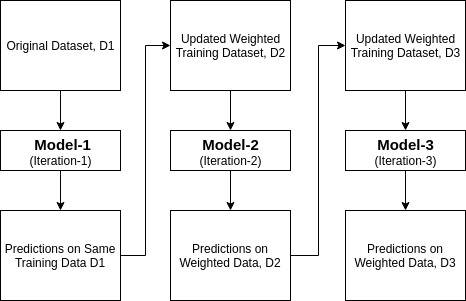
\includegraphics[width=0.85\linewidth]{figure/AdaBoost.jpg}
	\caption{AdaBoost流程}
	\label{fig:AdaBoost}
\end{figure}

\subsection{训练方法}

不同于普通的分类问题,本问题是一个Learning to Rank的模型,不能简单地套用AdaBoost算法。且我们在训练时使用的是pairwise training方法,而在预测时需要对所有推荐物品排序,这其中的差异使得AdaBoost的应用并不方便。

我做的一个尝试是:在训练时仍采用抽样-pairwise training-更新权重的方法。pairwise training中每个元组可视为一个二分类问题,目标是使得正样本的出现概率高于负样本。计算分类器误差时,若某一元组的概率大于$0.5$,则将其视为正确分类的样本。在分类时,将$K$个分类器的权重进行加权平均,后比较所有物品的权重,取其中最大的三个作为最终的推荐结果。该方法最终取得了比较好的效果。

\paragraph{参数设置}
受系统内存大小限制,我们无法使用较多的模型进行组合,故仅设置模型数量$K$为$5$。对于每个模型,设置其参数维度$d=90$,学习率为$0.0005$。每次训练的过程中,从整个训练样本中有放回的抽样$10,000,000$个样本。整个训练过程在服务器上持续了一个星期,也足以说明这个问题的规模之大。


%\newpage
\section{结果评估}

本节将汇报我的模型取得的成绩,同时说明整个提交文件的结构和测试模块的书写过程,以便助教进行检查。

\subsection{代码文件}

提交文件包括两部分:训练代码与测试文件。为了避免文件过大,中间产生的处理文件没有提交。文件说明如下:
\begin{enumerate}
\item {\bf train/Preprocess\_test.ipynb}:test数据集的处理程序,按照时间间隔将测试数据划分为Public和Private两部分。
\item {\bf train/Preprocess\_train.ipynb}:train数据集的预处理代码,对应第\ref{sec:session}节中的预处理过程。
\item {\bf train/Pairwise Preprocess.ipynb}:成对训练的数据处理程序,对应第\ref{sec:pair}节中的过程,处理出用于训练的样本对。
\item {\bf train/Trainer.ipynb}:基本LFM模型,未添加任何额外的因素。
\item {\bf train/Pairwise Training.ipynb}:成对训练方法,添加了所有衡量用户喜好的因素。
\item {\bf train/Duration.ipynb}:用户行为模型,一个失败的尝试,未被用到最终的模型中。
\item {\bf train/Adaboost.ipynb}:最终模型,融合了Pairwise Train和AdaBoost方法。
\end{enumerate}

{\bf 注1}:除Adaboost之外,其他的训练代码中都可能有些许的错误,因为是在写后面的算法时候才发现的,所以就没有在原文件里修改。

{\bf 注2}:以上代码中的参数设置均偏小,主要为了能让代码在我的笔记本上运行,便于检查代码正确性,所以未调大参数。实际训练中使用的参数请参照第\ref{sec:train}节。


\subsection{实验过程}
\label{sec:train}

整个实验过程总共持续了三个星期,其中有三次大的训练阶段:基本模型、成对训练和组合方法。主要是为了检验一下中间模型的性能,但是发现训练过程实在太耗时间,最后一次组合方法的训练整整持续了一个周。

\paragraph{电脑配置} 
因为模型中的参数量超过了1亿,且样本量巨大,我笔记本电脑的内存根本跑不动,于是就借了实验室的服务器来跑。服务器的配置是\textit{Intel i7-7700K @ 4.2-GHz (4 Cores)} \textit{32GB}内存。

\paragraph{正则化}
我们没有在最终训练过程中加入正则化项(论文中也没有),而是通过手动调整的方式进行。在每个epoch结束时,trainer会汇报当前epoch的平均正确率,当发现正确率可接受(85\%以上)时,中断训练,预测结果,这一过程可使用try...except语句实现。

\paragraph{训练参数}
最终训练时,我们设置模型个数$K=5$,属性向量的维度$d=90$,学习率为$0.0005$,其余参数均在正文中有汇报。

\subsection{测试模块}

因为比赛无法提交,所以我们只好由自己书写测试程序,再与标准答案进行对比。我根据第\ref{sec:submit}和\ref{sec:eval}节中的描述书写了测试程序存放在test/test.ipynb文件中。

测试的思路比较简单,按照答案中给出的Public和Private信息划分数据,然后进行统计即可。为了证明测试程序的正确性,我对example submission的得分进行了测试,结果如图~\ref{fig:sample}。

\begin{figure}[htbp]
	\centering
	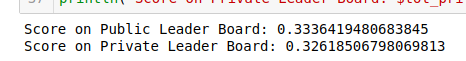
\includegraphics[width=0.85\linewidth]{figure/sample.png}
	\caption{tester计算出的样例测试结果}
	\label{fig:sample}
\end{figure}

而样例提交在LeaderBoard上的得分分别如图~\ref{fig:public}和~\ref{fig:private}所示。二者相同,可验证tester的正确性。

\begin{figure}[htbp]
	\centering
	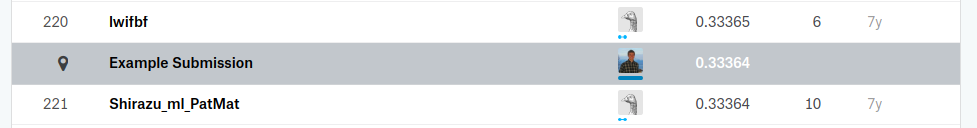
\includegraphics[width=\linewidth]{figure/public.png}
	\caption{Public Leaderboard上的样例测试结果}
	\label{fig:public}
\end{figure}

\begin{figure}[htbp]
	\centering
	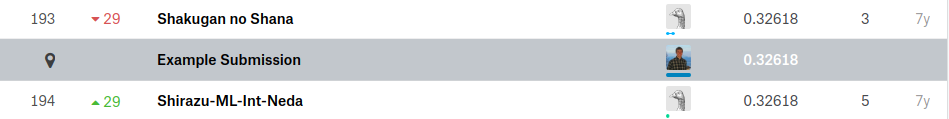
\includegraphics[width=\linewidth]{figure/private.png}
	\caption{Private Leaderboard上的样例测试结果}
	\label{fig:private}
\end{figure}


\subsection{测试结果}

最终,我的模型经过测试得到的分数为{\bf 0.42768(public score)/0.41811(private score)},在Public Leaderboard上{\bf 排名5/657},在Private Leaderboard上{\bf 排名3/657},测试结果如图~\ref{fig:test}所示。

\begin{figure}[htbp]
	\centering
	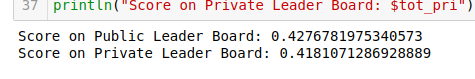
\includegraphics[width=0.85\linewidth]{figure/final.png}
	\caption{最终测试结果}
	\label{fig:test}
\end{figure}

为了证明得分的真实性,我将答案文件一并提交,存放在test/test.csv文件下,可通过运行test/tester.ipynb文件来验证答案的分数。

%\newpage
\section{结论}

在本项目中,我参考\cite{chen2012context}一文改进LFM模型,使用AdaBoost方法对KDD2012 Track1的推荐问题进行求解,最终取得了第3名的成绩。在打比赛的过程中,感悟颇深,尤其感受到数据挖掘过程中许多细小琐碎的问题,如数据预处理、参数的调整、实现错误导致浪费大量的训练时间等等。整个PJ的工作量十分巨大,整整耗费了我两个半周的时间,训练的过程也比较久。不过,总体来说,收获非常大,尤其是最后取得了比较不错的成绩(尽管没有原论文成绩好,可能是因为我没有完全理解论文中的做法)。希望以后还可以参加类似的数据挖掘比赛!




\newpage
\bibliographystyle{unsrt} 
\bibliography{PJ}

\section*{致谢}

\addcontentsline{toc}{section}{致谢}

\begin{itemize}
\item 感谢汪卫老师与肖仰华老师一学期的课程指导。
\item 感谢助教在我完成PJ中提供的宝贵建议。
\item 感谢张宇恒同学与我交流论文复现中的细节。
\end{itemize}




\end{sloppypar}
\end{document}
